\documentclass[12pt, twoside]{article}
\usepackage[francais]{babel}
\usepackage[T1]{fontenc}
\usepackage[latin1]{inputenc}
\usepackage[left=9mm, right=9mm, top=8mm, bottom=8mm]{geometry}
\usepackage{float}
\usepackage{graphicx}
\usepackage{array}
\usepackage{multirow}
\usepackage{amsmath,amssymb,mathrsfs}
\usepackage{soul}
\usepackage{textcomp}
\pagestyle{empty}
\begin{document}

\begin{flushright}
$2^{de}5$
\end{flushright}
\begin{center}
\textbf{\large{Devoir Maison 3}}
\end{center}

\textit{Devoir � rendre sur feuille double grand format petits carreaux pour le
\ul{jeudi 06 novembre 2008}.}

\textit{La qualit� de la r�daction et de la pr�sentation sont prises en compte
dans la notation.}



\bigskip
\textbf{Exercice 1:} 

\begin{center}
  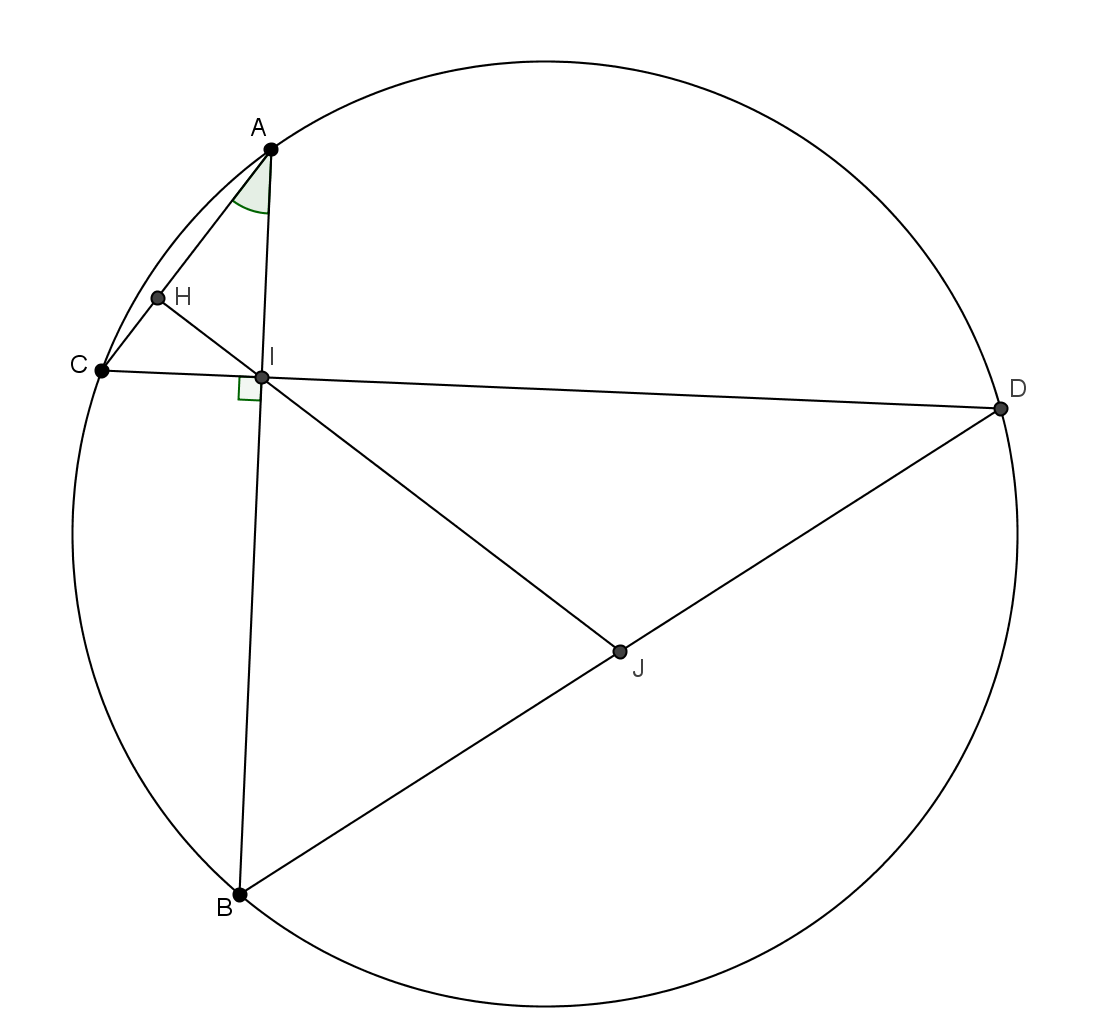
\includegraphics[width=7cm]{image/geogebra.png}
\end{center}


Sur la figure ci-contre, $A,B,C,D$ sont quatre points d'un cercle tels que les
droites $(AB)$ et $(CD)$ soient perpendiculaires. On note $I$ le point
d'intersection. Le point $J$ est le milieu du segment $[BD]$ et la droite $(IJ)$
coupe le segment $[AC]$ en $H$.

\begin{enumerate}
  \item L'angle $\widehat{IAC}$ mesure $35�$. Faire la figure sur
  \textbf{Geogebra} et l'enregistrer dans le \textbf{dossier ressource} de la
  classe avec le titre : "Nom-pr�nom-DM3-ex1"
  \item Evaluer tous les angles de la figure (avec le logiciel),les noter sur
  votre copie.
  \item Quelle conjecture peut-on faire sur l'angle $\widehat{IHA}$? (on ne
  demande pas la justification.)
\end{enumerate}

\bigskip
\bigskip




\textbf{Exercice 2:} Donner une valeur arrondie � $10^{-3}$ pr�s de la hauteur
d'un triangle �quilat�ral de $6\ cm$ de c�t�.


\medskip

\textit{Indication: Il est conseill� de faire une figure et de repr�senter la
hauteur (pour pouvoir donner une valeur approch�e, il faut d�j� conna�tre une
valeur exacte).}


\bigskip
\bigskip  
  
  
\textbf{Exercice 3:} 
\medskip 


\textit{Conseil: il est pr�f�rable de relire les
identit�s remarquables \ldots}

\medskip 
\begin{enumerate}
  \item Montrer qu'il est possible de calculer les carr�s qui suivent sans
  avoir recours � une calculatrice: $31^{2}$, $81^{2}$ et $59^{2}$.
  \item Montrer qu'il est possible de justifier que les nombres ci-dessous ne
  sont pas premiers sans avoirs recours � une calculatrice:
  $899 \thinspace 999 \thinspace 999 \thinspace 999 \thinspace 999$; \enskip
  $63 \thinspace 993 439$; \enskip  
  $224 \thinspace 999  \thinspace 999 \thinspace 999 \thinspace 039$; \enskip
  $899 \thinspace 999 \thinspace 999 \thinspace 996 \thinspace 519$; \enskip
  $1 \thinspace 599 \thinspace 999 \thinspace 999 \thinspace 999 \thinspace
  559$.
\end{enumerate}

\end{document}
